\chapter{Combinatoria}

\index{combinatoria}

La \key{combinatoria} estudia métodos para contar combinaciones de objetos.
Usualmente, el objetivo es encontrar una manera de contar las combinaciones
eficientemente sin generar cada combinación individualmente.

Para empezar, consideremos el problema de contar el número de maneras de
representar un entero $n$ como la suma de enteros positivos. Por ejemplo,
existen 8 representaciones para $4$:
\begin{multicols}{2}
    \begin{itemize}
        \item $1+1+1+1$
        \item $1+1+2$
        \item $1+2+1$
        \item $2+1+1$
        \item $2+2$
        \item $3+1$
        \item $1+3$
        \item $4$
    \end{itemize}
\end{multicols}

A menudo, los problemas combinatoriales pueden resolverse utilizando funciones
recursivas. En este problema, podemos definir una función $f(n)$ que devuelva
el número de representaciones para $n$. Por ejemplo, $f(4)=8$, como vimos en el
ejemplo anterior. Los valores de la función pueden calcularse recursivamente
de la siguiente manera:
\begin{equation*}
    f(n) = \begin{cases}
        1                       & n = 0 \\
        f(0)+f(1)+\cdots+f(n-1) & n > 0 \\
    \end{cases}
\end{equation*}
El caso base es $f(0)=1$, porque solo la suma vacía representa al número 0.
Si $n>0$, consideraremos todas las formas de elegir el primer número de
la suma. Si el primer número es $k$, existen $f(n-k)$ representaciones para
la parte restante de la suma. Entonces, calculamos la suma de todos los
valores con forma $f(n-k)$ donde $k<n$.

Los primeros valores para la función son:
\[
    \begin{array}{lcl}
        f(0) & = & 1 \\
        f(1) & = & 1 \\
        f(2) & = & 2 \\
        f(3) & = & 4 \\
        f(4) & = & 8 \\
    \end{array}
\]

A veces, una fórmula recursiva puede reemplazarse por una fórmula de forma
cerrada. En este problema,
\[
    f(n)=2^{n-1},
\]
que está basado en el hecho de que hay $n-1$ posiciones posibles para los
signos ``+'' en la suma y podemos elegir cualquier subconjunto de ellos.

\section{Coeficientes binomiales}

\index{coeficiente binomial}

El \key{coeficiente binomial} $\binom{n}{k}$ equivale al número de formas
posibles en las que podemos elegir un subconjunto de $k$ elementos a partir de
un conjunto de $n$ elementos. Por ejemplo, $\binom{5}{3}=10$, porque el conjunto
$\{1,2,3,4,5\}$ posee 10 subconjuntos de 3 elementos:
\[ \{1,2,3\}, \{1,2,4\}, \{1,2,5\}, \{1,3,4\}, \{1,3,5\},
    \{1,4,5\}, \{2,3,4\}, \{2,3,5\}, \{2,4,5\}, \{3,4,5\} \]

\subsubsection{Fórmula 1}

Los coeficientes binomiales pueden calcularse recursivamente de la siguiente
manera:

\[
    \binom{n}{k} = \binom{n-1}{k-1} + \binom{n-1}{k}
\]

La idea es fijar un elemento $x$ en el conjunto. Si $x$ está incluido en el
subconjunto, debemos elegir $k-1$ elementos a partir de $n-1$ elementos, y si
$x$ no está incluido, debemos elegir $k$ elementos a partir de $n-1$ elementos.

Los casos base para la recursión son
\[
    \binom{n}{0}  =  \binom{n}{n} = 1,
\]
porque siempre hay exactamente una forma de construir un subconjunto vacío
y un subconjunto que contiene todos los elementos.

\subsubsection{Fórmula 2}

Otra manera de calcular eficientes binomiales es la siguiente:
\[
    \binom{n}{k}  =  \frac{n!}{k!(n-k)!}.
\]

Hay $n!$ permutaciones de $n$ elementos. Recorremos todas las permutaciones y
siempre incluimos los primeros $k$ elementos de la permutación en el
subconjunto. Ya que el orden de los elementos en el subconjunto y fuera del
subconjunto es irrelevante, el resultado se divide por $k!$ y $(n-k)!$.

\subsubsection{Propiedades}

Para los coeficientes binomiales,
\[
    \binom{n}{k}  =  \binom{n}{n-k},
\]
porque realmente dividimos un conjunto de $n$ elementos en dos subconjuntos:
el primero contiene $k$ elementos y el segundo contiene $n-k$ elementos.

La suma de coeficientes binomiales es
\[
    \binom{n}{0}+\binom{n}{1}+\binom{n}{2}+\ldots+\binom{n}{n}=2^n.
\]

Podemos ver la razón del nombre ``coeficiente binomial'' cuando el binomio
$(a+b)$ se eleva a la $n$-ésima potencia:

\[ (a+b)^n =
    \binom{n}{0} a^n b^0 +
    \binom{n}{1} a^{n-1} b^1 +
    \ldots +
    \binom{n}{n-1} a^1 b^{n-1} +
    \binom{n}{n} a^0 b^n. \]

\index{triángulo de Pascal}

Los coeficientes binomiales también aparecen en el \key{triángulo de Pascal},
donde cada valor equivale a la suma de sus dos valores superiores:
\begin{center}
    \begin{tikzpicture}[scale=0.9]
        \node at (0,0) {1};
        \node at (-0.5,-0.5) {1};
        \node at (0.5,-0.5) {1};
        \node at (-1,-1) {1};
        \node at (0,-1) {2};
        \node at (1,-1) {1};
        \node at (-1.5,-1.5) {1};
        \node at (-0.5,-1.5) {3};
        \node at (0.5,-1.5) {3};
        \node at (1.5,-1.5) {1};
        \node at (-2,-2) {1};
        \node at (-1,-2) {4};
        \node at (0,-2) {6};
        \node at (1,-2) {4};
        \node at (2,-2) {1};
        \node at (-2,-2.5) {$\ldots$};
        \node at (-1,-2.5) {$\ldots$};
        \node at (0,-2.5) {$\ldots$};
        \node at (1,-2.5) {$\ldots$};
        \node at (2,-2.5) {$\ldots$};
    \end{tikzpicture}
\end{center}

\subsubsection{Cajas y bolas}

``Cajas y bolas'' es un modelo útil en donde contamos las formas de colocar
$k$ bolas en $n$ cajas. Consideremos tres situaciones:

\textit{Situación 1}: Cada caja puede contener a lo sumo una bola.
Por ejemplo, cuando $n=5$ y $k=2$, existen 10 soluciones:

\begin{center}
    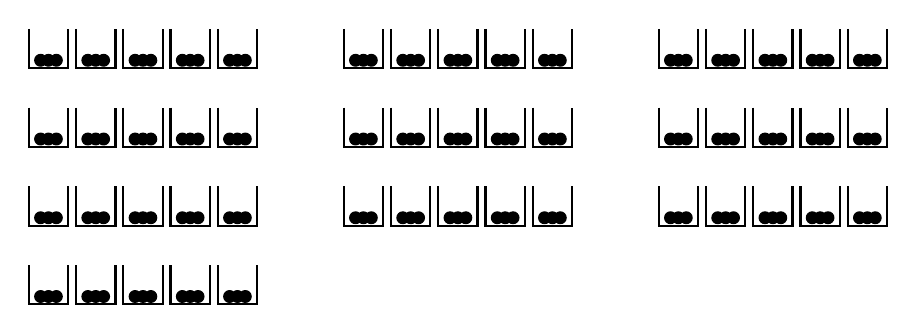
\begin{tikzpicture}[scale=0.5]
        \newcommand\lax[3]{
            \path[draw,thick,-] (#1-0.5,#2+0.5) -- (#1-0.5,#2-0.5) --
            (#1+0.5,#2-0.5) -- (#1+0.5,#2+0.5);
            \ifthenelse{\equal{#3}{1}}{\draw[fill=black] (#1,#2-0.3) circle (0.15);}{}
            \ifthenelse{\equal{#3}{2}}{\draw[fill=black] (#1-0.2,#2-0.3) circle (0.15);}{}
            \ifthenelse{\equal{#3}{2}}{\draw[fill=black] (#1+0.2,#2-0.3) circle (0.15);}{}
        }
        \newcommand\laa[7]{
            \lax{#1}{#2}{#3}
            \lax{#1+1.2}{#2}{#4}
            \lax{#1+2.4}{#2}{#5}
            \lax{#1+3.6}{#2}{#6}
            \lax{#1+4.8}{#2}{#7}
        }

        \laa{0}{0}{1}{1}{0}{0}{0}
        \laa{0}{-2}{1}{0}{1}{0}{0}
        \laa{0}{-4}{1}{0}{0}{1}{0}
        \laa{0}{-6}{1}{0}{0}{0}{1}
        \laa{8}{0}{0}{1}{1}{0}{0}
        \laa{8}{-2}{0}{1}{0}{1}{0}
        \laa{8}{-4}{0}{1}{0}{0}{1}
        \laa{16}{0}{0}{0}{1}{1}{0}
        \laa{16}{-2}{0}{0}{1}{0}{1}
        \laa{16}{-4}{0}{0}{0}{1}{1}

    \end{tikzpicture}
\end{center}

En esta situación, la respuesta es directamente el coeficiente binomial
$\binom{n}{k}$.

\pagebreak
\textit{Situación 2}: Una caja puede contener múltiples bolas. Por ejemplo,
cuando $n=5$ y $k=2$, existen 15 soluciones:

\begin{center}
    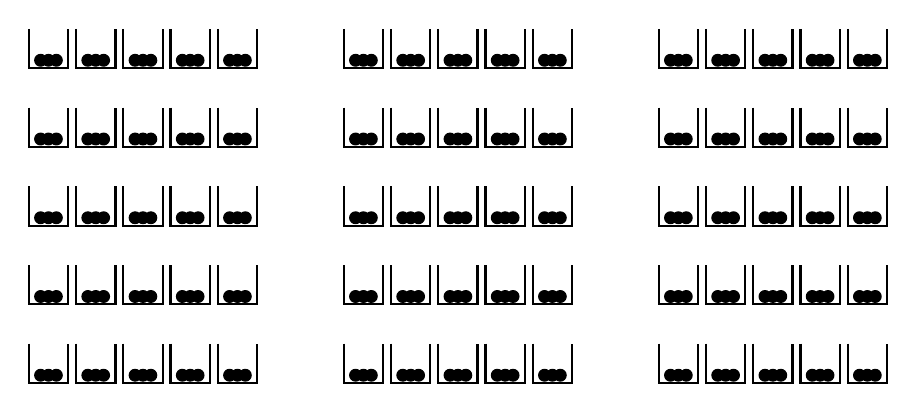
\begin{tikzpicture}[scale=0.5]
        \newcommand\lax[3]{
            \path[draw,thick,-] (#1-0.5,#2+0.5) -- (#1-0.5,#2-0.5) --
            (#1+0.5,#2-0.5) -- (#1+0.5,#2+0.5);
            \ifthenelse{\equal{#3}{1}}{\draw[fill=black] (#1,#2-0.3) circle (0.15);}{}
            \ifthenelse{\equal{#3}{2}}{\draw[fill=black] (#1-0.2,#2-0.3) circle (0.15);}{}
            \ifthenelse{\equal{#3}{2}}{\draw[fill=black] (#1+0.2,#2-0.3) circle (0.15);}{}
        }
        \newcommand\laa[7]{
            \lax{#1}{#2}{#3}
            \lax{#1+1.2}{#2}{#4}
            \lax{#1+2.4}{#2}{#5}
            \lax{#1+3.6}{#2}{#6}
            \lax{#1+4.8}{#2}{#7}
        }

        \laa{0}{0}{2}{0}{0}{0}{0}
        \laa{0}{-2}{1}{1}{0}{0}{0}
        \laa{0}{-4}{1}{0}{1}{0}{0}
        \laa{0}{-6}{1}{0}{0}{1}{0}
        \laa{0}{-8}{1}{0}{0}{0}{1}
        \laa{8}{0}{0}{2}{0}{0}{0}
        \laa{8}{-2}{0}{1}{1}{0}{0}
        \laa{8}{-4}{0}{1}{0}{1}{0}
        \laa{8}{-6}{0}{1}{0}{0}{1}
        \laa{8}{-8}{0}{0}{2}{0}{0}
        \laa{16}{0}{0}{0}{1}{1}{0}
        \laa{16}{-2}{0}{0}{1}{0}{1}
        \laa{16}{-4}{0}{0}{0}{2}{0}
        \laa{16}{-6}{0}{0}{0}{1}{1}
        \laa{16}{-8}{0}{0}{0}{0}{2}

    \end{tikzpicture}
\end{center}

El proceso de colocar bolas en las cajas puede representarse como una cadena
de caracteres ``$\circ$'' y ``$\rightarrow$''. Inicialmente, asumimos que nos
encontramos en la caja más a la izquierda. El símbolo ``$\circ$'' significa que
colocamos una bola en la caja actual, y el símbolo ``$\rightarrow$'' significa
que nos movemos a la siguiente caja derecha.

Utilizando esta notación, cada solución es una cadena que contiene $k$
veces el símbolo ``$\circ$'' y $n-1$ veces el símbolo ``$\rightarrow$''.
Por ejemplo, la solución de arriba a la derecha en la imagen anterior
corresponde a la cadena
``$\rightarrow \rightarrow \circ \rightarrow \circ \rightarrow$''.
Por lo tanto, el número de soluciones es $\binom{k+n-1}{k}$.

\textit{Situación 3}: Cada caja puede contener a lo sumo una bola y, además,
no pueden haber dos cajas adyacentes que contengan bolas. Por ejemplo, cuando
$n=5$ y $k=2$, existen 6 soluciones:

\begin{center}
    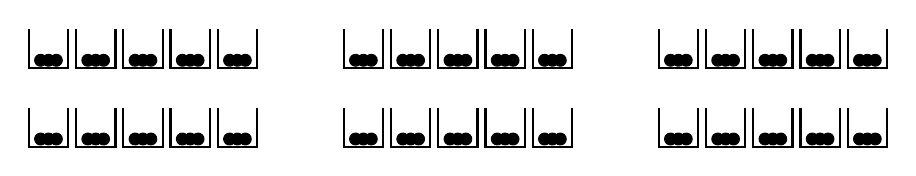
\begin{tikzpicture}[scale=0.5]
        \newcommand\lax[3]{
            \path[draw,thick,-] (#1-0.5,#2+0.5) -- (#1-0.5,#2-0.5) --
            (#1+0.5,#2-0.5) -- (#1+0.5,#2+0.5);
            \ifthenelse{\equal{#3}{1}}{\draw[fill=black] (#1,#2-0.3) circle (0.15);}{}
            \ifthenelse{\equal{#3}{2}}{\draw[fill=black] (#1-0.2,#2-0.3) circle (0.15);}{}
            \ifthenelse{\equal{#3}{2}}{\draw[fill=black] (#1+0.2,#2-0.3) circle (0.15);}{}
        }
        \newcommand\laa[7]{
            \lax{#1}{#2}{#3}
            \lax{#1+1.2}{#2}{#4}
            \lax{#1+2.4}{#2}{#5}
            \lax{#1+3.6}{#2}{#6}
            \lax{#1+4.8}{#2}{#7}
        }

        \laa{0}{0}{1}{0}{1}{0}{0}
        \laa{0}{-2}{1}{0}{0}{1}{0}
        \laa{8}{0}{1}{0}{0}{0}{1}
        \laa{8}{-2}{0}{1}{0}{1}{0}
        \laa{16}{0}{0}{1}{0}{0}{1}
        \laa{16}{-2}{0}{0}{1}{0}{1}
    \end{tikzpicture}
\end{center}

En esta situación, podemos asumir que hay $k$ bolas inicialmente colocadas
en cajas y existe una caja vacía entre cada par de cajas adyacentes. Ahora
queda elegir las posiciones para las cajas vacías restantes. Existen
$n-2k+1$ tales cajas y $k+1$ posiciones para ellas. Por lo tanto, usando la
fórmula de la situación 2, el número de soluciones es $\binom{n-k+1}{n-2k+1}$.

\subsubsection{Coeficientes multinomiales}

\index{coeficiente multinomial}

El \key{coeficiente multinomial}
\[ \binom{n}{k_1,k_2,\ldots,k_m} = \frac{n!}{k_1! k_2! \cdots k_m!}, \]
equivale al número de formas en las que podemos dividir $n$ elementos en
subconjuntos de tamaños $k_1,k_2,\ldots,k_m$, donde $k_1+k_2+\cdots+k_m=n$.
Podemos ver a los coeficientes multinomiales como una generalización de los
coeficientes binomiales; si $m=2$, la fórmula de arriba corresponde a la
fórmula del coeficiente binomial.

\section{Números de Catalan}

\index{número de Catalan}

El \key{número de Catalan} $C_n$ equivale al número de expresiones de
paréntesis válidas que consistan de $n$ paréntesis izquierdas y $n$
paréntesis derechas.

Por ejemplo, $C_3=5$, porque podemos construir las siguientes expresiones de
paréntesis usando tres paréntesis izquierdas y tres derechas:

\begin{itemize}[noitemsep]
    \item \texttt{()()()}
    \item \texttt{(())()}
    \item \texttt{()(())}
    \item \texttt{((()))}
    \item \texttt{(()())}
\end{itemize}

\subsubsection{Expresiones de paréntesis}

\index{expresión de paréntesis}

¿Qué es exactamente una \emph{expresión de paréntesis válida}? Las siguientes
reglas definen precisamente todas las expresiones de paréntesis válidas:

\begin{itemize}
    \item Una expresión de paréntesis vacía es válida.
    \item Si una expresión $A$ es válida, entonces también es válida la
          expresión \texttt{(}$A$\texttt{)}.
    \item Si dos expresiones $A$ y $B$ son válidas, también es
          válida la expresión $AB$.
\end{itemize}

Otra manera de caracterizar expresiones de paréntesis válidas es que si
elegimos cualquier prefijo de tal expresión, debe contener por lo menos
tantas paréntesis izquierdas como derechas. Adicionalmente, la expresión
completa debe contener un número igual de paréntesis izquierdas y derechas.

\subsubsection{Fórmula 1}

Los números de Catalan pueden calcularse utilizando la fórmula
\[ C_n = \sum_{i=0}^{n-1} C_{i} C_{n-i-1}.\]

La suma recorre todas las maneras de dividir la expresión en dos partes tal
que ambas partes sean expresiones válidas y la primera parte sea tan pequeña
como sea posible, pero no vacía. Para cualquier $i$, la primera parte contiene
$i+1$ pares de paréntesis y el número de expresiones es el producto de los
siguientes valores:

\begin{itemize}
    \item $C_{i}$: el número de formas de construir una expresión
          usando las paréntesis de la primera parte, sin contar
          las paréntesis más externas
    \item $C_{n-i-1}$: el número de formas de construir una expresión
          usando las paréntesis de la segunda parte
\end{itemize}

El caso base es $C_0=1$, porque podemos construir una expresión válida
utilizando cero pares de paréntesis.

\subsubsection{Fórmula 2}

Los números de Catalan también pueden calcularse utilizando coeficientes
binomiales:
\[ C_n = \frac{1}{n+1} \binom{2n}{n}\]
La fórmula puede entenderse de la siguiente manera:

Hay un total de $\binom{2n}{n}$ maneras de construir una expresión de
paréntesis (no necesariamente válida) que contenga $n$ paréntesis izquierdos
y $n$ paréntesis derechos. Calculemos el número de tales expresiones que
\emph{no} sean válidas.

Si una expresión de paréntesis no es válida, debe contener un prefijo donde
el número de paréntesis derechos exceda el número de paréntesis izquierdos.
La idea es invertir cada paréntesis que pertenezca a tal prefijo. Por ejemplo,
la expresión \texttt{())()(} contiene un prefijo \texttt{())}, y luego de
invertir el prefijo, la expresión se vuelve \texttt{)((()(}.

La expresión resultante consiste de $n+1$ paréntesis izquierdos y $n-1$
paréntesis derechos. El número de tales expresiones es $\binom{2n}{n+1}$,
que equivale al número de expresiones de paréntesis inválidas. Por lo tanto,
el número de expresiones válidas puede calcularse usando la fórmula
\[\binom{2n}{n}-\binom{2n}{n+1} = \binom{2n}{n} - \frac{n}{n+1} \binom{2n}{n} = \frac{1}{n+1} \binom{2n}{n}.\]

\subsubsection{Contar árboles}

Los números de Catalan también se relacionan con los árboles:

\begin{itemize}
    \item existen $C_n$ árboles binarios de $n$ nodos
    \item existen $C_{n-1}$ árboles con raíz de $n$ nodos
\end{itemize}
\noindent
Por ejemplo, para $C_3=5$, los árboles binarios son

\begin{center}
    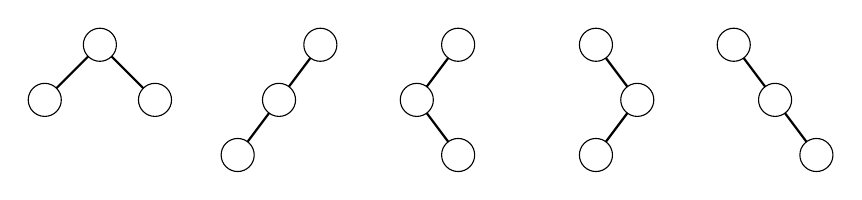
\begin{tikzpicture}[scale=0.7]
        \path[draw,thick,-] (0,0) -- (-1,-1);
        \path[draw,thick,-] (0,0) -- (1,-1);
        \draw[fill=white] (0,0) circle (0.3);
        \draw[fill=white] (-1,-1) circle (0.3);
        \draw[fill=white] (1,-1) circle (0.3);

        \path[draw,thick,-] (4,0) -- (4-0.75,-1) -- (4-1.5,-2);
        \draw[fill=white] (4,0) circle (0.3);
        \draw[fill=white] (4-0.75,-1) circle (0.3);
        \draw[fill=white] (4-1.5,-2) circle (0.3);

        \path[draw,thick,-] (6.5,0) -- (6.5-0.75,-1) -- (6.5-0,-2);
        \draw[fill=white] (6.5,0) circle (0.3);
        \draw[fill=white] (6.5-0.75,-1) circle (0.3);
        \draw[fill=white] (6.5-0,-2) circle (0.3);

        \path[draw,thick,-] (9,0) -- (9+0.75,-1) -- (9-0,-2);
        \draw[fill=white] (9,0) circle (0.3);
        \draw[fill=white] (9+0.75,-1) circle (0.3);
        \draw[fill=white] (9-0,-2) circle (0.3);

        \path[draw,thick,-] (11.5,0) -- (11.5+0.75,-1) -- (11.5+1.5,-2);
        \draw[fill=white] (11.5,0) circle (0.3);
        \draw[fill=white] (11.5+0.75,-1) circle (0.3);
        \draw[fill=white] (11.5+1.5,-2) circle (0.3);
    \end{tikzpicture}
\end{center}
y los árboles con raíz son
\begin{center}
    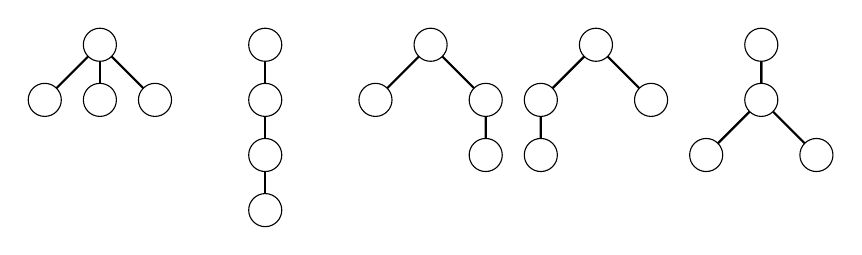
\begin{tikzpicture}[scale=0.7]
        \path[draw,thick,-] (0,0) -- (-1,-1);
        \path[draw,thick,-] (0,0) -- (0,-1);
        \path[draw,thick,-] (0,0) -- (1,-1);
        \draw[fill=white] (0,0) circle (0.3);
        \draw[fill=white] (-1,-1) circle (0.3);
        \draw[fill=white] (0,-1) circle (0.3);
        \draw[fill=white] (1,-1) circle (0.3);

        \path[draw,thick,-] (3,0) -- (3,-1) -- (3,-2) -- (3,-3);
        \draw[fill=white] (3,0) circle (0.3);
        \draw[fill=white] (3,-1) circle (0.3);
        \draw[fill=white] (3,-2) circle (0.3);
        \draw[fill=white] (3,-3) circle (0.3);

        \path[draw,thick,-] (6+0,0) -- (6-1,-1);
        \path[draw,thick,-] (6+0,0) -- (6+1,-1) -- (6+1,-2);
        \draw[fill=white] (6+0,0) circle (0.3);
        \draw[fill=white] (6-1,-1) circle (0.3);
        \draw[fill=white] (6+1,-1) circle (0.3);
        \draw[fill=white] (6+1,-2) circle (0.3);

        \path[draw,thick,-] (9+0,0) -- (9+1,-1);
        \path[draw,thick,-] (9+0,0) -- (9-1,-1) -- (9-1,-2);
        \draw[fill=white] (9+0,0) circle (0.3);
        \draw[fill=white] (9+1,-1) circle (0.3);
        \draw[fill=white] (9-1,-1) circle (0.3);
        \draw[fill=white] (9-1,-2) circle (0.3);

        \path[draw,thick,-] (12+0,0) -- (12+0,-1) -- (12-1,-2);
        \path[draw,thick,-] (12+0,0) -- (12+0,-1) -- (12+1,-2);
        \draw[fill=white] (12+0,0) circle (0.3);
        \draw[fill=white] (12+0,-1) circle (0.3);
        \draw[fill=white] (12-1,-2) circle (0.3);
        \draw[fill=white] (12+1,-2) circle (0.3);

    \end{tikzpicture}
\end{center}

\section{Inclusión--exclusión}

\index{inclusion--exclusión}

La \key{inclusión--exclusión} es una técnica que puede utilizarse para
contar el tamaño de una unión de conjuntos cuando los tamaños de las
intersecciones son conocidos, y vice versa. Un simple ejemplo de la
técnica es la fórmula
\[ |A \cup B| = |A| + |B| - |A \cap B|,\]
donde $A$ y $B$ son conjuntos y $|X|$ denota el tamaño de $X$. La fórmula
puede ilustrarse de la siguiente manera:

\begin{center}
    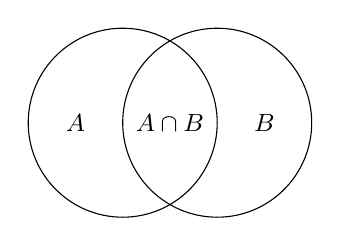
\begin{tikzpicture}[scale=0.8]

        \draw (0,0) circle (1.5);
        \draw (1.5,0) circle (1.5);

        \node at (-0.75,0) {\small $A$};
        \node at (2.25,0) {\small $B$};
        \node at (0.75,0) {\small $A \cap B$};

    \end{tikzpicture}
\end{center}

Nuestro objetivo es calcular el tamaño de la unión $A \cup B$ que corresponde
al área de la región que pertenece a por lo menos menos un círculo. La imagen
muestra que podemos calcular el área de $A \cup B$ si primero sumamos las
áreas de $A$ y $B$ y luego restamos el área de $A \cap B$.

La misma idea es aplicable cuándo el número de conjuntos es mayor. Cuando
hay tres conjuntos, la fórmula de inclusión--exclusión es
\[ |A \cup B \cup C| = |A| + |B| + |C| - |A \cap B|  - |A \cap C|  - |B \cap C| + |A \cap B \cap C| \]
y la imagen correspondiente es

\begin{center}
    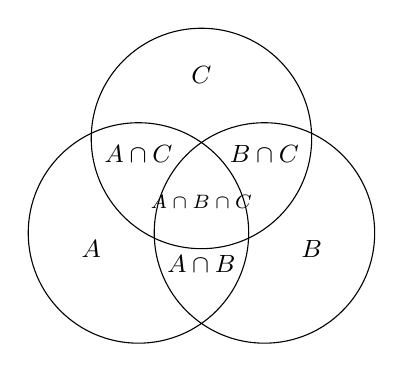
\begin{tikzpicture}[scale=0.8]

        \draw (0,0) circle (1.75);
        \draw (2,0) circle (1.75);
        \draw (1,1.5) circle (1.75);

        \node at (-0.75,-0.25) {\small $A$};
        \node at (2.75,-0.25) {\small $B$};
        \node at (1,2.5) {\small $C$};
        \node at (1,-0.5) {\small $A \cap B$};
        \node at (0,1.25) {\small $A \cap C$};
        \node at (2,1.25) {\small $B \cap C$};
        \node at (1,0.5) {\scriptsize $A \cap B \cap C$};

    \end{tikzpicture}
\end{center}

En el caso general, el tamaño de la unión $X_1 \cup X_2 \cup \cdots \cup X_n$
puede calcularse recorriendo todas las posibles intersecciones que contengan
alguno(s) de los conjuntos $X_1,X_2,\ldots,X_n$. Si la intersección contiene
un número impar de conjuntos, su tamaño es sumado al resultado, y de lo
contrario su tamaño es restado del mismo.

Ten en cuenta que hay fórmulas similares para calcular el tamaño de una
intersección a partir de los tamaños de las uniones. Por ejemplo,
\[ |A \cap B| = |A| + |B| - |A \cup B|\]
y
\[ |A \cap B \cap C| = |A| + |B| + |C| - |A \cup B|  - |A \cup C|  - |B \cup C| + |A \cup B \cup C| .\]

\subsubsection{Desarreglos}

\index{desarreglo}

Como ejemplo, contemos el número de \key{desarreglos} de los elementos
$\{1,2,\ldots,n\}$, o sea, las permutaciones donde ningún elemento permanece
en su lugar original. Por ejemplo, cuando $n=3$, existen dos desarreglos:
$(2,3,1)$ y $(3,1,2)$.

Un método para resolver el problema es utilizar la inclusión--exclusión.
Definamos $X_k$ como el conjunto de permutaciones que contienen el elemento
$k$ en la posición $k$. Por ejemplo, cuando $n=3$, los conjuntos son:
\[
    \begin{array}{lcl}
        X_1 & = & \{(1,2,3),(1,3,2)\} \\
        X_2 & = & \{(1,2,3),(3,2,1)\} \\
        X_3 & = & \{(1,2,3),(2,1,3)\} \\
    \end{array}
\]
Usando estos conjuntos, el número de desarreglos equivale a
\[ n! - |X_1 \cup X_2 \cup \cdots \cup X_n|, \]
por lo que es suficiente calcular el tamaño de la unión. Utilizando la
inclusión--exclusión, esto se reduce a calcular tamaños de intersecciones,
algo que podemos hacer eficientemente. Por ejemplo, cuando $n=3$, el tamaño de
$|X_1 \cup X_2 \cup X_3|$ es
\[
    \begin{array}{lcl}
         &   & |X_1| + |X_2| + |X_3| - |X_1 \cap X_2|  - |X_1 \cap X_3|  - |X_2 \cap X_3| + |X_1 \cap X_2 \cap X_3| \\
         & = & 2+2+2-1-1-1+1                                                                                        \\
         & = & 4,                                                                                                   \\
    \end{array}
\]
así que el número de soluciones $3!-4=2$.

Resulta que el problema también puede resolverse sin usar la
inclusión--exclusión. Definamos $f(n)$ como el número de desarreglos para
$\{1,2,\ldots,n\}$. Podemos usar la siguiente fórmula recursiva:

\begin{equation*}
    f(n) = \begin{cases}
        0                      & n = 1 \\
        1                      & n = 2 \\
        (n-1)(f(n-2) + f(n-1)) & n>2   \\
    \end{cases}
\end{equation*}

Podemos derivar la fórmula si consideramos las posibilidades de cómo cambia
el elemento 1 en el desarreglo. Hay $n-1$ maneras de elegir un elemento $x$
que reemplace al elemento 1. En cada elección tal, existen dos opciones:

\textit{Opción 1}: También reemplazamos el elemento $x$ por el elemento 1.
Luego de esto, la tarea restante es construir un desarreglo de $n-2$ elementos.

\textit{Opción 2}: Reemplazamos el elemento $x$ por algún otro que 1.
Ahora debemos construir un desarreglo de $n-1$ elementos, porque no podemos
reemplazar el elemento $x$ con el elemento $1$, y todos los otros elementos
deben cambiarse.

\section{Lema de Burnside}

\index{lema de Burnside}

El \key{lema de Burnside} puede utilizarse para contar el número de
combinaciones tal que solo un representante es utilizado para cada grupo
de combinaciones simétricas. El lema de Burnside establece que el número
de combinaciones es
\[\sum_{k=1}^n \frac{c(k)}{n},\]
cuando hay $n$ formas de cambiar la posición de una combinación, y hay
$c(k)$ combinaciones que permanecen iguales cuando la $k$-ésima forma
es aplicada.

Por ejemplo, calculemos el número de collares con $n$ perlas, donde cada
perla tiene $m$ colores posibles. Dos collares son simétricos si son similares
tras ser rotados. Por ejemplo, el collar
\begin{center}
    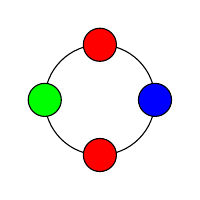
\begin{tikzpicture}[scale=0.7]
        \draw[fill=white] (0,0) circle (1);
        \draw[fill=red] (0,1) circle (0.3);
        \draw[fill=blue] (1,0) circle (0.3);
        \draw[fill=red] (0,-1) circle (0.3);
        \draw[fill=green] (-1,0) circle (0.3);
    \end{tikzpicture}
\end{center}
tiene los siguientes collares simétricos:
\begin{center}
    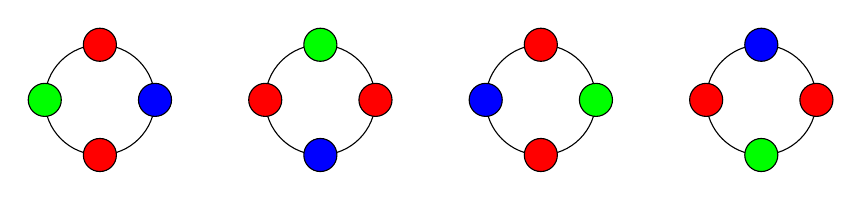
\begin{tikzpicture}[scale=0.7]
        \draw[fill=white] (0,0) circle (1);
        \draw[fill=red] (0,1) circle (0.3);
        \draw[fill=blue] (1,0) circle (0.3);
        \draw[fill=red] (0,-1) circle (0.3);
        \draw[fill=green] (-1,0) circle (0.3);

        \draw[fill=white] (4,0) circle (1);
        \draw[fill=green] (4+0,1) circle (0.3);
        \draw[fill=red] (4+1,0) circle (0.3);
        \draw[fill=blue] (4+0,-1) circle (0.3);
        \draw[fill=red] (4+-1,0) circle (0.3);

        \draw[fill=white] (8,0) circle (1);
        \draw[fill=red] (8+0,1) circle (0.3);
        \draw[fill=green] (8+1,0) circle (0.3);
        \draw[fill=red] (8+0,-1) circle (0.3);
        \draw[fill=blue] (8+-1,0) circle (0.3);

        \draw[fill=white] (12,0) circle (1);
        \draw[fill=blue] (12+0,1) circle (0.3);
        \draw[fill=red] (12+1,0) circle (0.3);
        \draw[fill=green] (12+0,-1) circle (0.3);
        \draw[fill=red] (12+-1,0) circle (0.3);
    \end{tikzpicture}
\end{center}
Existen $n$ formas de cambiar la posición de un collar, porque podemos rotarlo
$0,1,\ldots,n-1$ pasos en sentido horario. Si el número de pasos es 0, todos
los $m^n$ collares permanecen iguales, y si el número de pasos es 1, solo los
$m$ collares donde cada perla tiene el mismo color permanecen iguales.

Más generalmente, donde el número de pasos es $k$, un total de
\[m^{\textrm{mcd}(k,n)}\]
collares permanecen iguales, donde $\textrm{mcd}(k,n)$ es el máximo común
divisor de $k$ y $n$. La razón es que bloques de perlas de tamaño
$\textrm{mcd}(k,n)$ se reemplazarán el uno al otro. Por lo tanto, según el
lema de Burnside, el número de collares es
\[\sum_{i=0}^{n-1} \frac{m^{\textrm{mcd}(i,n)}}{n}. \]
Por ejemplo, el número de collares de tamaño 4 con 3 colores es
\[\frac{3^4+3+3^2+3}{4} = 24. \]

\section{Fórmula de Cayley}

\index{fórmula de!Cayley}

La \key{fórmula de Cayley} dice que existen $n^{n-2}$ árboles con etiquetas
que contengan $n$ nodos. Los nodos están etiquetados $1,2,\ldots,n$, y dos
árboles son diferentes si ya sea su estructura o etiquetado es diferente.

\pagebreak
Por ejemplo, cuando $n=4$, el número de árboles etiquetados es $4^{4-2}=16$:

\begin{center}
    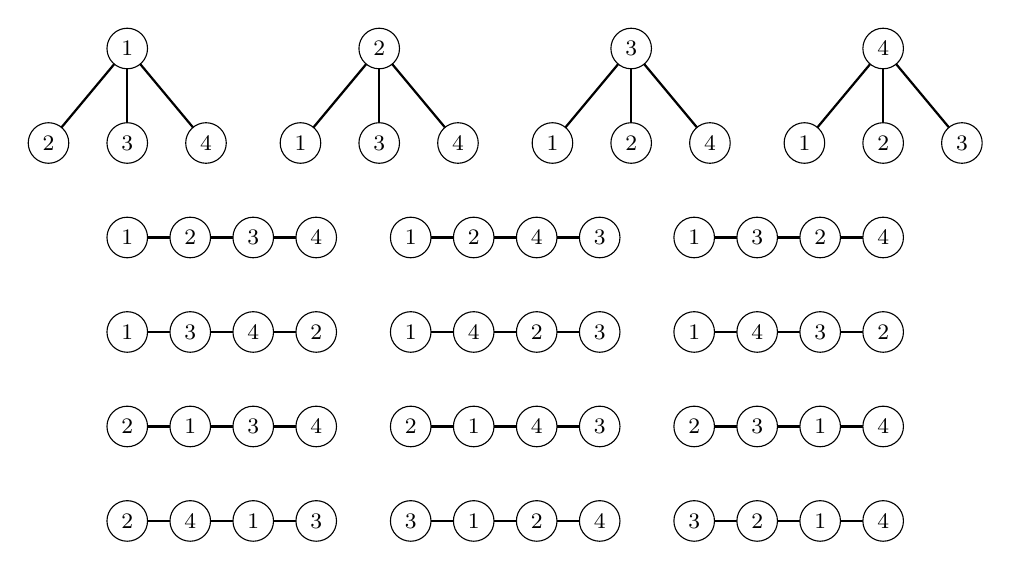
\begin{tikzpicture}[scale=0.8]
        \footnotesize

        \newcommand\puua[6]{
            \path[draw,thick,-] (#1,#2) -- (#1-1.25,#2-1.5);
            \path[draw,thick,-] (#1,#2) -- (#1,#2-1.5);
            \path[draw,thick,-] (#1,#2) -- (#1+1.25,#2-1.5);
            \node[draw, circle, fill=white] at (#1,#2) {#3};
            \node[draw, circle, fill=white] at (#1-1.25,#2-1.5) {#4};
            \node[draw, circle, fill=white] at (#1,#2-1.5) {#5};
            \node[draw, circle, fill=white] at (#1+1.25,#2-1.5) {#6};
        }
        \newcommand\puub[6]{
            \path[draw,thick,-] (#1,#2) -- (#1+1,#2);
            \path[draw,thick,-] (#1+1,#2) -- (#1+2,#2);
            \path[draw,thick,-] (#1+2,#2) -- (#1+3,#2);
            \node[draw, circle, fill=white] at (#1,#2) {#3};
            \node[draw, circle, fill=white] at (#1+1,#2) {#4};
            \node[draw, circle, fill=white] at (#1+2,#2) {#5};
            \node[draw, circle, fill=white] at (#1+3,#2) {#6};
        }

        \puua{0}{0}{1}{2}{3}{4}
        \puua{4}{0}{2}{1}{3}{4}
        \puua{8}{0}{3}{1}{2}{4}
        \puua{12}{0}{4}{1}{2}{3}

        \puub{0}{-3}{1}{2}{3}{4}
        \puub{4.5}{-3}{1}{2}{4}{3}
        \puub{9}{-3}{1}{3}{2}{4}
        \puub{0}{-4.5}{1}{3}{4}{2}
        \puub{4.5}{-4.5}{1}{4}{2}{3}
        \puub{9}{-4.5}{1}{4}{3}{2}
        \puub{0}{-6}{2}{1}{3}{4}
        \puub{4.5}{-6}{2}{1}{4}{3}
        \puub{9}{-6}{2}{3}{1}{4}
        \puub{0}{-7.5}{2}{4}{1}{3}
        \puub{4.5}{-7.5}{3}{1}{2}{4}
        \puub{9}{-7.5}{3}{2}{1}{4}
    \end{tikzpicture}
\end{center}

Ahora veremos cómo derivar la fórmula de Cayley con códigos de Prüfer.

\subsubsection{Código de Prüfer}

\index{código de Prüfer}
\index{secuencia de Prüfer}

Un \key{código de Prüfer} es una secuencia de $n-2$ números que describen
un árbol etiquetado. El código es construido siguiendo un proceso que remueve
$n-2$ hojas del árbol. En cada paso, la hoja con la etiqueta más pequeña es
quitada, y la etiqueta de su único vecino es añadida al código.

Por ejemplo, calculemos el código de Prüfer del siguiente grafo:
\begin{center}
    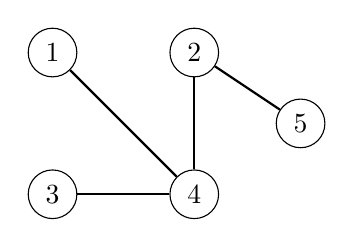
\begin{tikzpicture}[scale=0.9]
        \node[draw, circle] (1) at (2,3) {$1$};
        \node[draw, circle] (2) at (4,3) {$2$};
        \node[draw, circle] (3) at (2,1) {$3$};
        \node[draw, circle] (4) at (4,1) {$4$};
        \node[draw, circle] (5) at (5.5,2) {$5$};

        \path[draw,thick,-] (1) -- (4);
        \path[draw,thick,-] (3) -- (4);
        \path[draw,thick,-] (2) -- (4);
        \path[draw,thick,-] (2) -- (5);
    \end{tikzpicture}
\end{center}

Primero quitamos el nodo 1 y añadimos el nodo 4 al código:
\begin{center}
    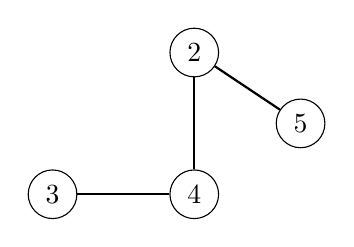
\begin{tikzpicture}[scale=0.9]
        %\node[draw, circle] (1) at (2,3) {$1$};
        \node[draw, circle] (2) at (4,3) {$2$};
        \node[draw, circle] (3) at (2,1) {$3$};
        \node[draw, circle] (4) at (4,1) {$4$};
        \node[draw, circle] (5) at (5.5,2) {$5$};

        %\path[draw,thick,-] (1) -- (4);
        \path[draw,thick,-] (3) -- (4);
        \path[draw,thick,-] (2) -- (4);
        \path[draw,thick,-] (2) -- (5);
    \end{tikzpicture}
\end{center}

Luego quitamos el nodo 3 y añadimos el nodo 4 al código:
\begin{center}
    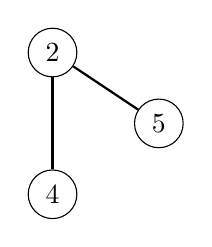
\begin{tikzpicture}[scale=0.9]
        %\node[draw, circle] (1) at (2,3) {$1$};
        \node[draw, circle] (2) at (4,3) {$2$};
        %\node[draw, circle] (3) at (2,1) {$3$};
        \node[draw, circle] (4) at (4,1) {$4$};
        \node[draw, circle] (5) at (5.5,2) {$5$};

        %\path[draw,thick,-] (1) -- (4);
        %\path[draw,thick,-] (3) -- (4);
        \path[draw,thick,-] (2) -- (4);
        \path[draw,thick,-] (2) -- (5);
    \end{tikzpicture}
\end{center}

Finalmente quitamos el nodo 4 y añadimos el nodo 2 al código:
\begin{center}
    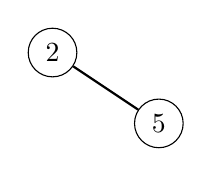
\begin{tikzpicture}[scale=0.9]
        %\node[draw, circle] (1) at (2,3) {$1$};
        \node[draw, circle] (2) at (4,3) {$2$};
        %\node[draw, circle] (3) at (2,1) {$3$};
        %\node[draw, circle] (4) at (4,1) {$4$};
        \node[draw, circle] (5) at (5.5,2) {$5$};

        %\path[draw,thick,-] (1) -- (4);
        %\path[draw,thick,-] (3) -- (4);
        %\path[draw,thick,-] (2) -- (4);
        \path[draw,thick,-] (2) -- (5);
    \end{tikzpicture}
\end{center}

Finalmente, el código de Prüfer del grafo es $[4,4,2]$.

Podemos construir un código de Prüfer para cualquier árbol y, que es más
importante, el árbol original puede ser reconstruido a partir de un
código de Prüfer. Por lo tanto, el número de árboles etiquetados de $n$ nodos
equivale a $n^{n-2}$, el número de códigos de Prüfer de tamaño $n$.
